%% Author_tex.tex
%% V1.0
%% 2012/13/12
%% developed by Techset
%%
%% This file describes the coding for rsproca.cls

\documentclass[]{rsos}%%%%where rsos is the template name
\usepackage{multirow}
\usepackage{float}
\usepackage{lineno}
\linenumbers

%%%% *** Do not adjust lengths that control margins, column widths, etc. ***

\begin{document}

%%%% Article title to be placed here
\title{Idiosyncratic patterns of chromosome evolution are the rule not the exception}

\author{%%%% Author details
Terrence Sylvester$^{1}$, Carl E. Hjelmen$^{1}$, J. Spencer Johnston$^{2}$, and Heath Blackmon$^{1}$}

%%%%%%%%% Insert author address here
\address{$^{1}$Department of Biology; Texas A\&M University; College Station, TX 77843, USA\\
$^{2}$Department of Entomology; Texas A\&M University; College Station, TX 77843, USA}


%%%% Subject entries to be placed here %%%%
\subject{Evolutionary Biology}

%%%% Keyword entries to be placed here %%%%
\keywords{fusion, fission, chromosome number, sex chromosome, Polyneoptera, karyotype}

%%%% Insert corresponding author and its email address}
\corres{Heath Blackmon\\
\email{blackmon@tamu.edu}}

%%%% Abstract text to be placed here %%%%%%%%%%%%
\modulolinenumbers[1]
\begin{internallinenumbers}
\begin{abstract}
The structure of a genome can be described at its simplest by the number of chromosomes and the sex chromosome system it contains. 
Despite over a century of study, the evolution of genome structure on this scale remains recalcitrant to broad generalisations that can be applied across clades. 
To address this issue, we have assembled a dataset of 823 karyotypes from the insect group Polyneoptera. 
This group contains orders with a range of variations in chromosome number, and offer the opportunity to explore the possible causes of these differences.
We have analysed this data using both phylogenetic and taxonomic approaches.
Our analysis allows us to assess the importance of rates of evolution, phylogenetic history, sex chromosome systems, parthenogenesis, and genome size on variation in chromosome number within clades. 
We find that fusions play a key role in the origin of new sex chromosomes, and that orders exhibit striking differences in rates of fusions, fissions, or polyploidy.
Our results suggest that the difficulty in finding consistent rules that govern evolution at this scale may be due to the presence of many interacting forces that can lead to variation among groups.
\end{abstract}
%%%%%%%%%%%%%%%%%%%%%%%%%%%

%%%%%%%%%% Insert the texts which can accomdate on firstpage in the tag "fmtext" %%%%%

\begin{fmtext}
\section{Introduction}
Chromosome number is one of the fundamental characteristics of a genome.
It is also the first information collected about most genomes. 
In fact, the first chromosome counts were recorded prior to the development of the chromosome theory of inheritance \cite{flemming1882}.
Despite this early start, consistent rules governing the evolution of chromosome number across large clades remain elusive.



\end{fmtext}
\end{internallinenumbers}
%%%%%%%%%%%%%%% End of first page %%%%%%%%%%%%%%%%%%%%%

\maketitle

Changes in chromosome number can happen due to several mechanisms.
We use the term fusion and fission to describe respectively a decrease or an increase of one in chromosome number.
However, these terms are simplifications and may represent multiple processes at the molecular level.
Reduction in chromosome number can happen through Robertsonian translocations with the loss of nonessential DNA \cite{garagna1995}.
Reductions can also happen through the fusion of two chromosomes at the telomeres followed by loss of one of the centromeres \cite{gordon2011mechanisms, miga2016}.
In contrast, increases in chromosome number can occur due to simple chromosome fission in the centromere region \cite{moretti1984}.
Increases in chromosome number can also happen due to the duplication of an entire chromosome.
Changes in chromosome number of more than one can also occur.
Although rare in most animal groups, demiploidy describes an increase chromosome number by one-half. 
Demiploidy events can occur by the joining of haploid gamete with an unreduced diploid gamete \cite{hornsey1973}.
Finally, whole-genome duplication can lead to a doubling of chromosome number \cite{beccak1970}.

These changes in chromosome number can have broad impacts on gene transcription, recombination rates, and sex chromosome evolution.
Presence of an extra copy of a chromosome can lead to both increases and decreases in gene transcription.  
For instance, the presence of a third copy of a chromosome can lead to approximately a four per cent increase in gene expression across all chromosomes and a 1.5-fold increase in expression of genes on that chromosome \cite{lockstone2007, williams2008aneuploidy}.
In \textit{Drosophila} females with three X chromosomes, expression of genes in each X chromosome is reduced such that the total X chromosome gene expression matches with that of females with two X chromosomes \cite{sun2013dosage}.
However, the presence of an extra copy of the X chromosome in \textit{Drosophila} females leads to a 33\% reduction in the expression of genes on the autosomes \cite{sun2013dosage}. 

It has long been recognised that chromosome number should positively correlate with genome-wide recombination rates \cite{stebbins1958}.
The frequency of recombination events and the proper segregation of chromosomes into gametes is dependent on crossing over in meiosis.
The lower limit of the number of crossing over events is controlled by the number of chromosome arms in most species and by the number of chromosomes in some species \cite{dumont2017req}.
This relationship between chromosome number and recombination has been suggested as a source of indirect selection on chromosome number in Hymenoptera though recent analysis suggest this may be only a weak force \cite{ross2015, sherman1979}.
Reduced recombination between loci (due to a fusion between an autosome and the sex chromosomes --- reducing chromosome number) has been implicated in the speciation of the Japan Sea stickleback \cite{kitano2012}. 

Changes in chromosome number can have impacts on the evolution and behaviour of sex chromosomes. 
For instance, if chromosomes are broken into smaller chromosomes while keeping all else equal (e.g. genome size), the average chromosome size should be negatively correlated with the number of chromosomes.
This can have important impacts on the fate of sex chromosomes.
A comparative study of Coleoptera has shown that species are more likely to lose the Y chromosome and transition from XY to XO if they have many small chromosomes rather than a few larger chromosomes \cite{blackmon2015bioessay}.
It has been hypothesized that this pattern is driven by the size of the region available for recombination between the X and Y chromosome during male meiosis and the frequency that males will produce aneuploid gametes \cite{blackmon2014}.
However, in some species, this may be averted by cell cycle checkpoints that lead to apoptosis of cells that fail to properly segregate the sex chromosomes \cite{dumont2017par}.

In sexual species, it is often assumed that changes in chromosome number are underdominant--heterozygotes have reduced fitness \cite{white1973} . 
Chromosomal heterozygosity occurs when the chromosome
% TS: changed compliment to complement. - reply for R2.2
\textcolor{red}{\st{compliment}} \textcolor{blue}{complement} from the parents differs.
For instance, if one parent contributes a single fused chromosome and the other contributes two separate chromosomes.
Perhaps the most widely known example of this is hybridisation between horses and donkeys where the offspring carries 32 chromosomes from the mother and 31 chromosomes from the father. 
When this mule attempts to produce gametes the rearrangements that have occurred lead to gametes lacking a full set of all genes in the genome and thus, they are sterile \cite{wodsedalek1916}. 
It should be noted that this fitness reduction is not always observed.
In wild mice which are heterozygous for a single fusion between chromosomes 16 and 17, there is no significant reduction in fertility and thus no reduction in fitness \cite{britton1990robertsonian}.
A large number of crosses in lemurs (where the chromosome number ranged from 44 to 60) exhibit a full range of fitness effects of changes in chromosome number.
Four of twelve hybrids exhibit normal spermatogenesis while six of twelve exhibits reduced spermatogenesis while the final two hybrids exhibited major perturbations to spermatogenesis \cite{ratomponirina1988}.   
In contrast, one can hypothesise that changes in chromosome number might be less deleterious in asexual species since they do not have to pair with any other genome in the population.
Consistent with this asexual species have considerable variation in chromosome number.
In parthenogenetic beetle species, we find polyploid races within species where the total chromosome number of polyploid races is a multiple of the haploid number.
For example, in weevils (Coleoptera: Curculionidae), the species \textit{Catapionus gracilicornis} has polyploid races with chromosome numbers of 22, 33, 44 and 55 \cite{lachowska1998}. 

To better understand the dynamics of chromosome evolution we have chosen to work with the insect clade Polyneoptera which includes commonly known groups such as termites, grasshoppers, and cockroaches.
This group contains the orders Blattodea (including Isoptera), Dermaptera, Embiidina, Mantodea, Notoptera, Orthoptera, Phasmatodea, and Plecoptera.
\textcolor{blue}{Polyneoptera show striking differences in chromosome number variation among orders, and one of the central goals of this study was to determine if these differences are due to unique rates and patterns of evolution in each order or due simply to differences in the phylogenetic history of the orders.
Polyneoptera also have variation in sex chromosome systems (i.e. XX/XO, XX/XY or complex XY) and, include sexual and asexual species allowing us to explore interactions between these characteristics and the evolution of chromosome number.
We have assembled a large trait dataset of chromosome number, Sex Chromosome System (SCS), genome size, and reproductive mode.}
We analysed this data in both a taxonomic and a phylogenetic framework to determine the impact of the sexual system on rates of chromosome number evolution, the source of transitions in SCSs, and identify differences in patterns of chromosome number evolution across orders.

\section{Material and methods}

\subsection{Chromosome data}
We downloaded all available chromosome data for the clade Polyneoptera from the Tree of Sex database \cite{blackmon2016,TOS2014}.
To supplement this data, we performed literature searches for each order in Polyneoptera.
Briefly, we combined order names with the terms "cytogenetic", "cytotaxonomic", "karyotype", and "sex chromosome system".
For each species in our dataset, we made an attempt to score three traits: chromosome number, SCS, and reproductive mode (sexual vs. asexual).
In cases where there were multiple records for a species that had different values, we retained all reported values.
This process yielded a final dataset of 823 records, 773 of which are unique taxa, with the remaining records representing species that have variability in one of the recorded traits (Table S1).

\subsection{Phylogenetic data}
We used PyPHLAWD to retrieve sequence clusters and used clusters which had at least 100 species for our analysis \cite{smith2018phyphlawd}. 
These included three mitochondrial genes (COI, COX2 and ND4) and three nuclear
% TS: changed 18s and 28s to 18S and 28S - reply for R1.2
regions (\textcolor{red}{\st{18s}} \textcolor{blue}{18S} and two regions of the \textcolor{red}{\st{28s}} \textcolor{blue}{28S} gene). 
We removed duplicate sequences and retained the longest example for each species using the function FastaFilter in the R package evobiR \cite{blackmon2015evobir}.
To maximise the overlap between our trait and sequence datasets we first found all species-level exact matches in both datasets.
% TS: changed genera level and genus level to genus-level and species level to species-level - reply for R2.4
Next, we looked for \textcolor{red}{\st{genera level}} \textcolor{blue}{genus-level} matches that lacked \textcolor{red}{\st{species level}} \textcolor{blue}{species-level} matches.
For each of these \textcolor{red}{\st{genus level}} \textcolor{blue}{genus-level} matches, we retained the longest sequence for each locus from any species in the genus and used these sequences to act as a tip representing the genus rather than any single species. 
This process of maximising the overlap between the two datasets created 57 exemplar taxa (genera tips).

We used MAFFT under default settings to align all sequences \cite{katoh2013mafft}.
For the aligned RNA coding sequences, we used GBLOCKS to remove hypervariable regions \cite{castresana2000gblocks}. 
When running GBLOCKS, we used default settings with the exception of the allowed gap positions argument which was set to maximum. 
For the 18S sequence cluster, we also set the minimum block length to 6 to retain a greater proportion of the alignment. 
For the protein-coding genes, we manually adjusted the starting position of the alignments to maintain the reading frame. 
Using the supermatrix function in the R package evobiR, individual gene alignments were then concatenated into a supermatrix with 7380 sites \cite{blackmon2015evobir}.

The presence of rogue taxa (taxa that have an inconsistent placement in a set of phylogenetic trees) can produce unreliable rate inferences similar to that found in analyses of supertrees \cite{aberer2012roguetaxa, rabosky2015b}.
To identify the presence of rogue taxa, we generated 100 maximum likelihood rapid bootstrap trees using RAxML v 8.2.10 implemented in CIPRES Science Gateway \cite{stamatakis2014raxml,miller2010cipres}.
Using these trees, we calculated the taxonomic instability index as implemented in Mesquite v 3.51 \cite{maddison2018mesquite}.
When we examined taxonomic instability indices, we found that a score of 4870 was an inflexion point (Figure S1).
We identified 16 taxa whose taxonomic instability index was higher and removed them from subsequent analysis.
Our final alignment contained 232 taxonomic units with 73\% missing data.

We used BEAST v 2.5 \cite{bouckaert2014beast} to infer time-calibrated phylogenies under a relaxed lognormal clock, a birth-death model, and GTR + G as the nucleotide substitution model.
The mitochondrial and nuclear coding genes were partitioned into all three coding positions. 
We used previous estimates for the ages of seven nodes (Table S2) in our phylogeny drawn from a previous study of divergence times across insects \cite{misof2014phylogenomics}.
For each of these calibration points, we used a normal distribution.
The upper and lower bounds of the calibration points (95\textsuperscript{th} and 5\textsuperscript{th} percentiles respectively) were placed according to the confidence intervals as presented in Misof et al. \cite{misof2014phylogenomics}. 
We conducted two independent runs, each for 100 million generations.
The convergence of these two independent runs was evaluated using Tracer v 1.7 \cite{rambaut2018tracer}.
The initial 50\% of each MCMC run was discarded as burnin and 50 phylogenetic trees were randomly sampled from the post-burnin period of each run to construct a posterior distribution of 100 trees used for trait analyses described below.

The presence of parthenogenetic taxa in our dataset allows us to ask how reproductive mode affects chromosome number evolution.
However, the parthenogenetic mode of reproduction is only present in Phasmatodea.
Therefore we built a second phylogeny, for Phasmatodea, that included more species from our trait dataset.
To do this we supplemented the sequence data from PyPHLAWD with additional data located using the PhyLoTA web server \cite{sanderson2008}.
This increased our samples from 28 species, which we had in Polyneoptera dataset, to 41 species. 
This new dataset included three mitochondrial genes (16s, COI, COX2) and three
% TS: changed 18s and 28s to 18S and 28S - reply for R1.2
nuclear genes (\textcolor{red}{\st{18s}} \textcolor{blue}{18S}, \textcolor{red}{\st{28s}} \textcolor{blue}{28S} and H3).
The new alignment consisted of 57\% missing data.
We inferred time-calibrated phylogenies as described above.

\subsection{Modeling chromosome evolution}
\textcolor{blue}{There has been a proliferation of probabilistic models of chromosome evolution in the last several years.
Each of these has slightly different goals and approaches.
The first of these was Chromevol which focuses on estimates of rates and ancestral conditions within single clades and allows for Bayesian and maximum likelihood approaches to parameter estimation \cite{mayrose2009chromevol, glick2014chromevol}.
The base model implemented in Chromevol has been expanded to more complex models like chromeploid which focuses on evolution of polyploidy and interactions between chromosome number and binary traits and performs parameter estimation in a maximum likelihood framework \cite{zenil2018chromploid}.
Two other extended models have been implemented in a Bayesian framework; ChromeSSE which compares cladogenetic and anagentic models of evolution \cite{freyman2018}, and chromePlus which focuses on the interactions between chromosome number and binary traits and allows for the binary trait to impact rates of diversification \cite{blackmon2019meiotic}. 
For the purposes of our investigation chromePlus was the most appropriate because of the flexibility offered within a Bayesian analysis and its ability to account for interactions between chromosome number evolution and binary traits\cite{blackmon2019meiotic}.}
To get reliable estimates for the rates of chromosome number evolution, we only analysed the four orders with at least 20 representatives.
We tested two versions of our model, a simple model with chromosome fission and fusion and a complex model which included fission, fusion, and polyploidy.
Although we use the terms fusion and fission for convenience, it should be noted that these are simply changes (decreases and increases respectively) in the haploid number by one.
Based on the likelihood ratio test results, we used the complex model to estimate the rates of chromosome evolution.

To account for uncertainty in chromosome number (e.g., when there were reports of multiple values for a tip in our phylogeny), we randomly sampled among the possible values.
This random sampling was repeated for each tree that we analysed.
To account for uncertainty in phylogeny, we ran an MCMC of 1000 generations for each of the 100 trees drawn from the posterior distribution.
Inspection of the parameter estimates revealed that our MCMC runs converged by 50 generations in most cases.  
We conservatively discarded the initial 25\% (250 states) as burnin and randomly sampled 100 states from the post-burnin portion of the run. 
This process yielded 10,000 point estimates that define the posterior distribution of the parameters in our model.
We tested for differences in rates of chromosome evolution by comparing the 95\% credible interval of the posterior distribution for each parameter in our model.
Rates were inferred with branch lengths transformed to make trees unit length.
However, all rates reported have been back-transformed so they represent transition rates in units of millions of years. 
% TS: added a sentence on the rate parameters to explain that the rate parameters that we describe here are waiting times for a transition to occur. - reply for R1.10
\textcolor{blue}{As is customary for Markov models the reported rates are lambda parameters for exponential distributions that describe the waiting time for a transition to occur.
Since our tree has branch lengths in units of millions of years these are reported in units of per MYA.}

\subsection{Genome size}
\textcolor{blue}{We also tested whether genome size as a proxy for repetitive content might explain variation in rate of chromosome number evolution among orders. 
Expansions in genome size are largely due to repetitive content, especially transposable elements \cite{kidwell2002transposable,bennetzen2005mechanisms}.
We reasoned that increased transposon activity could lead to a greater frequency of fusion and fission mutations and result in higher rates of chromosome number evolution in larger genomes.
We have also tested for a correlation between genome size and chromosome number, reasoning that recent whole genome duplications should lead to an increase in both values.
When multiple records for genome size for a species were available we used the mean value.
In the analysis of chromosome number and genome size we included genus level data where genome size and chromosome number were available for a genus but for different species within the genus.
We downloaded genome size data for all available species in Polyneoptera from the animal genome size database \cite{gregory2019}.
When multiple values for a single species were present the mean of each species was used.
Existing data was supplemented with new genome size estimates performed on 60 polyneoptera species using the flow cytometric method as found in Johnston et al. 2019 \cite{johnston2019}. 
Briefly, neural tissue was dissected from each insect and placed into Galbraith buffer for co-preparation with the \textit{Periplaneta americana} standard (1C = 3,338 Mbp) \cite{hanrahan2011}.
Tissue was ground gently with a Kontes ‘loose’ A pestle approximately 10-15 times before filtered through 41 micron filter.  Samples were stained for at least 30 minutes with 25µg/ml Propidium iodide before running through a Partec Cyflow SL 3 Flow cytometer with a 532 nm green laser. 
Samples were run to assure at least 1,000 nuclei under each 2C peak.
To test whether the mean genome size for an order predicted the mean rate estimate for chromosome gains, losses, and polyploidy a linear model was fit using the R function lm \cite{R-citation}.
To test whether genome size for species predicted chromosome number we created two linear models. 
The first, using all available data (N=53) was not phylogenetically corrected, and was fit with the lm function in R.
The second, used the subset of data which could be mapped to our phylogeny (N=19), and was fit with the phylolm function in the package phylolm which allows us to account for phylogenetic history \cite{R-citation, phylolm}.}

\subsection{Ancestral state reconstructions}
% TS: added recap on the traits on which we inferred the ancestral states. - reply for R1.6
\textcolor{blue}{We estimated the ancestral states of two traits; chromosome number and the sex chromosome system (SCS).}
We estimated the ancestral states of the chromosome number at the root of each orders using ChromEvol v 2.0. \cite{glick2014chromevol, mayrose2009chromevol}.
We used a fixed parameter model which included chromosome gains, losses, and whole-genome duplication---matching the model used in ChromePlus.
For each tree from our posterior distribution, we took the mean of each parameter estimate from the corresponding post-burnin portion of the ChromPlus analysis described above and supplied these to infer ancestral states in ChromEvol.
We integrated the estimates from the analysis of all 100 trees for each order to generate an ancestral state estimate that accounts for uncertainty in phylogeny and tip states. 

The estimate of ancestral states for SCSs was done using a Markov model in the function ACE in the R package APE \cite{Paradis2018}.
We classified multi-XY SCS as XY which resulted in two states (XO and XY) for the ancestral states reconstruction of the SCS. 
Our model allowed for transitions between XO and XY to occur at unequal rates.
To estimate the number of transitions in SCSs, we created the same model and performed stochastic mappings in the R package phytools \cite{revell2012phytools}.
Data and all R code for analyses are provided in a GitHub repository: https://github.com/Tsylvester8/Polyneoptera. 
% TS: added a sentence to talk about the polyneoptera karyotype database - reply for R1.7
\textcolor{blue}{The karyotype data can also be found in the Polyneoptera karyotype database at www.karyotype.org}

%%%%%%%%%%%%%
%% Results %%
%%%%%%%%%%%%%
\section{Results}

\subsection{Evolution of sex chromosome systems}
In our dataset, 21 genera contain species with different types of SCSs (i.e. XO XY, and or multi-XY).
In each of these genera, we calculated the mean autosome number for all species with a given type of SCS.
By comparing these means within genera, we can determine if differences are consistent with fusions or fissions as a source of transitions among SCSs.
Briefly, if transitions from XO to XY are generated by the fusion of an autosome to a sex chromosome we would expect a lower mean autosome number for XY species.
Likewise, if transitions from XY to multi-XY are generated by the fusion of an autosome to a sex chromosome we would expect a lower mean chromosome number for multi-XY species.
In contrast, if transitions from XY to multi-XY are generated by the fission of a sex chromosome we would expect no difference in the number of autosomes.

We find strong support for fusions as a source of transitions from XO to XY SCSs.
Of the 16 genera with both XO and XY species, 94\% (16/17) show a lower mean chromosome number in XY species (Table \ref{tab:fusions}). 
However, we find support for both fusions and fissions leading to transitions from XY to multi-XY.
While 43\% (3/7) of the genera with both XY and multi-XY have a higher mean autosome number in multi-XY species, 57\% (4/7) of the genera with both XY and multi-XY have a higher mean autosome number in XY species.
This analysis is limited to only those genera with variation in SCSs and thus omits much of our data.
When autosome number among orders is parsed by SCS, differences suggests that in some groups the origin of transitions may differ from our
% TS: changed genera level and genus level to genus-level and species level to species-level - reply for R2.4
\textcolor{red}{\st{genus level}} \textcolor{blue}{genus-level} analysis.
For instance, the mean of all XY species in both Blattodea (including Isoptera) and Dermaptera is higher than the mean of XO species in both orders.
This pattern is not expected if fusions are the primary source of transitions from XO to XY in these groups (Figure S2).

\subsection{Ancestral states and rates of sex chromosome evolution}

We find that the ancestral state for SCS in Polyneoptera clade was XO, with a probability of 90.3\%.
Similarly, the most probable ancestral state for each order was also XO, except for Isoptera and Dermaptera where XY is more probable (Fig. \ref{fig:sex.asr.plot}).
We find that the credible interval of the transition rates from XO to XY and XY to XO to be largely overlapping with means of 0.00202 and 0.00200 respectively. 
To assess the number of transitions between XY and XO we calculated the number of transitions from 100 stochastic maps for each of the 100 trees from the posterior sample.
Transitions from XO to XY were more common (mean = 15.3) while transitions from XY to XO were relatively rare (mean = 6.7).

\subsection{Chromosome number variation}
We find a significant difference in variance in chromosome numbers among the orders of Polyneoptera (Levene's test p-value: 2.2e-16). 
Blattodea (including Isoptera) (n = 172), had the highest variance in chromosome number (39.32) and  Embiidina (n = 8), had the lowest variance in chromosome number (0.41).
Orthoptera, despite having 319 records, had a low variance in chromosome number (2.87). 
Posthoc tests showed that Blattodea (including Isoptera) had a higher variance in chromosome number than Embiidina, Mantodea, Orthoptera, Phasmatodea, and Plecoptera (all p-values $<$ 0.05). 
Likewise, Dermaptera had a higher variance in chromosome number than Mantodea and Orthoptera (all p-values $<$ 0.05). Finally, Orthoptera had a lower variance in chromosome number than Phasmatodea (p-value $<$ 0.05).
Much of these differences in variance are obvious even when looking at the reduced phylogenetic dataset in Fig. \ref{fig:phyloplot}.

\subsection{Chromosome Number Evolution Rate inference}
Though differences in chromosome number variance suggest some orders are evolving more quickly, we must control for the phylogeny in order to draw any rigorous conclusions.
To do this we used a probabilistic model of chromosome evolution that can accommodate fusions, fissions, and whole genome duplications.
We began with a base model that includes only fusions and fissions and compared this via a likelihood ratio test with a model that included polyploidy as well.
We repeated this likelihood ratio test on each of the 100 trees from our posterior distribution for each order.
All orders showed some support for the model including polyploidy and overall, 77.6\% of our likelihood ratio tests supported the more complex model that included polyploidy.
For this reason, all analyses were done with a model that had fusions, fissions, and polyploidy.
In Blattodea (including Isoptera), we estimate a mean fusion rate of 0.128, a fission rate of 0.150, and a polyploidy rate of 0.003 (Table S3).
In contrast, if we remove the subclade Isoptera from Blattodea we find that parameter estimates increase to 0.420, 0.385, and 0.004 for fusions, fissions and polyploidy respectively.
This is consistent with rate estimates for Isoptera in isolation, where we infer
% TS: added a comma after 0.063 - reply for R2.7
a mean fusion rate of 0.044, a fission rate of \textcolor{red}{\st{0.063 and a polyploidy rate}} \textcolor{blue}{0.063, and a polyploidy rate} of 0.003.
In Mantodea, we estimate a mean fusion rate of 0.142, a fission rate of 0.056, and a polyploidy rate of 0.139.
Mantodea rate estimates also exhibited high uncertainty, overlapping rate estimates in most orders for most parameters (Fig. \ref{fig:order.rates.95HPD}, Figure S3).
In Phasmatodea, we estimate a mean fusion rate of 0.47, a fission rate of 0.145, and a polyploidy rate of 0.039.
Some of the lowest rates we estimated were in Orthoptera where the fusion rate was 0.003 and the fission rate was 0.024. However, we do find the polyploidy rate to be relatively high with a mean rate of 0.101.

% TS: new section on genome size
\subsection{Chromosome number evolution vs genome size}
Genome size data were available for 123 Polyneoptera species in the orders Phasmatodea, Orthoptera, Mantodea, and Blattodea (including Isoptera) in the genome size data base. We added additional 60 new genome size estimates to this existing dataset. These new estimates are now reported in Table Sxxx.
Mean genome size of these orders ranged from a low of 1.23 Gbp in Isoptera to a high of 7.92 Gbp in Orthoptera (Table S4).
% TS: changed rate of chromosome evolution to rate of chromosome number evolution. - reply for R1.8
We fit three linear models where the mean \textcolor{red}{\st{rate of chromosome evolution}} \textcolor{blue}{rate of chromosome number evolution} (gains, losses, and polyploidy) were a function of the mean genome size of an order.
None of these linear models was significant (all p-values $>$ 0.15 without correction for multiple comparisons).
Furthermore, some of the very lowest rates were observed in Orthoptera which had the largest mean genome size.
% TS: added the results on the correlation between the genome size and the chromosome number. - reply for editors comment on the power of our analysis on genome size and rate of chromosome number evolution.
\textcolor{blue}{In our comparison between genome size and chromosome number, we did not find any significant relationship as well (p values both before and after correcting for phylogeny were > 0.05) (Figure SX).}

\subsection{Chromosome Number Ancestral state reconstruction}
Prior to the application of probabilistic models of chromosome evolution the ancestral chromosome number was often assumed to be the most common chromosome number in extant species \cite{white1973}.
In reporting ancestral chromosome number in each order, we averaged probabilities across all 100 trees from the posterior distribution. 
Our analysis of Orthoptera \textcolor{blue}{(modal chromosome number 12)} suggests six is the most probable ancestral state for the order, with a 75.1\% probability.
However, a chromosome number of three is given a probability of 24.5\% which may suggest an early whole-genome duplication in this clade.
Support for the lower ancestral state was concentrated in 19 trees where the most probable state was 3 in all other trees 6 was given the highest probability (Figure S4).
In Blattodea including Isoptera \textcolor{blue}{(modal  chromosome number 21)}, the most probable chromosome number was 13 with a probability of 20.9\% followed by 14 and 12 with probabilities 19.5\% and 16.4\% respectively. 
In Blattodea excluding Isoptera \textcolor{blue}{(modal chromosome number 19)}, the most probable chromosome number was 7 with a probability of 11.9\% followed by 8 and 9 with probabilities 11.6\% and 11.2\% respectively.
In Isoptera \textcolor{blue}{(modal chromosome number 21)}, the most probable chromosome number was 20 with a probability of 35.6\% followed by 21 and 22 with probabilities 30.7\% and 14.0\% respectively.
In Mantodea \textcolor{blue}{modal chromosome number 14)}, the most probable chromosome number was 8 with a probability of 41.2\% followed by 9 and 7 with probabilities 19.2\% and 16.1\% respectively.
Finally, in Phasmatodea \textcolor{blue}{modal chromosome number 18)}, the most probable chromosome number was 9 with a probability of 11.7\% followed by 10 and 11 with probabilities 11.3\% and 10.7\% respectively.
\textcolor{blue}{All chromosome numbers reported here are haploid counts.}

\subsection{Asexuality and rates of chromosome number evolution}
Our dataset contains 13 parthenogenetic species.
All these species were within Phasmatodea.
Using our expanded Phasmatodea phylogenies we tested whether the rates of chromosome evolution are contingent on the reproductive mode (Figure S5).
We found that there is no significant difference in the rates of chromosome fusion and fission between sexually and asexually reproducing species.
However, we find that rates of polyploidy are significantly higher in asexually reproducing species than in sexually reproducing species (Fig. \ref{fig:phas.plot}).

%%%%%%%%%%%%%%%%
%% Discussion %%
%%%%%%%%%%%%%%%%
\section{Discussion}

The evolution of chromosome number across large clades and long time spans is fundamental to the diversity of genomes we observe across the tree of life.
Despite this, we are only beginning to understand how chromosome number evolves.
In this study, we have focused on the dynamics of chromosome evolution in Polyneoptera. 
Our analyses have revealed that this clade originated from an XO ancestor. 
We find that fusions have led to many new XY and multi-XY systems, and that only a few instances of fissions producing multi-XY systems appear to have occurred.
% TS: changed rate of chromosome evolution to rate of chromosome number evolution. - reply for R1.8
We see a rapid decline in the \textcolor{red}{\st{rate of chromosome evolution}} \textcolor{blue}{rate of chromosome number evolution} that coincides with the origin of eusocial Blattodea (Isoptera).
This is the opposite of the pattern documented in Hymenoptera \cite{ross2015}.
In Phasmatodea, we find that transitions into parthenogenetic reproduction allow for a high rate of polyploidy but no significant increase in rates of dysploidy.

\subsection{Sex chromosomes and chromosomes number evolution}
The transition between SCSs from XO to XY can occur through X chromosome autosome fusions or by sex chromosome turnover with fixation of the ancestral X
% TS: added citations. reply for R2.9
as a new autosome\textcolor{blue}{\cite{charlesworth1980, white1973}}.
Transition via fusion will lead to a reduction in the total number of autosomes, while turnover should lead to an increase in the total number of autosomes.
The data that we have collected shows a clear pattern of reduced autosome number in taxa with recent XO to XY transitions (Table \ref{tab:fusions}).
Transition from XY to multi-XY can occur through sex chromosome autosome fusions or by sex chromosome fission.
Transition via fusion will lead to a reduction in the total number of autosomes while fissions will lead to no change in the autosome number.
In contrast to the pattern observed in XO to XY transitions, transitions from XY to multi-XY show a mixed pattern with some having increased autosome number and some having decreased autosome number in taxa with recent XY to multi-XY transitions (Table \ref{tab:fusions}).
We interpret this as evidence for both fusions and fissions as an important source of multi-XY systems.
These SCS transitions could be neutral and fix simply due to drift or sexually antagonistic variation on autosome may lead to positive selection for increasing proportions of the genome becoming sex-linked through fusions \cite{charlesworth1980, kitano2012}.
Combining our results for XO to XY and XY to multi-XY transitions we find that fusions are a dominant route for changes in SCSs a pattern consistent with common sexual antagonistic variation on autosomes leading to selection for fusions. 

Our assembled data can also help us understand the fate of the Y chromosomes. 
It has been suggested that Y chromosomes may be destined to decay and loss given the inevitability of mutation accumulation due to lack of recombination \cite{steinemann2005}.
Alternatively, they may be retained through cycles of rejuvenation or even transitions into alternative forms of meiosis \cite{blackmon2015bioessay}.
In our inference of SCS evolution, we performed stochastic mappings that allow us to estimate the rate of Y chromosome loss and the number of inferred losses in our dataset.
The rate of Y chromosome gains and Y chromosome losses are both approximately 0.002 (Table S5). 
However, we find that Y chromosome gains are more common with a mean of 15.3 while losses are relatively rare with a mean of 6.7. 
This pattern is intuitive when we consider that the ancestor of this group was likely XO and thus there has been relatively little time for the gain of the Y chromosome to then be followed by its decay and loss.
% TS: added information on the support for common origin of the XO sex chromosome system in Polyneoptera. - reply for R2.8
\textcolor{blue}{Additionally, coupled with the evidence that X chromosome of German cockroach, \textit{Blattella germanica} (Blattodea), is highly conserved over 400 million years we suggest that the X chromosome in Polyneoptera species with XO sex chromosome system had a common origin \cite{meisel2019x}.}

\subsection{Eusociality and chromosome number}
In our analysis of Blattodea (including Isoptera), we inferred a significantly
% TS: changed rate of chromosome evolution to rate of chromosome number evolution. - reply for R1.8
lower \textcolor{red}{\st{rate of chromosome evolution}} \textcolor{blue}{rate of chromosome number evolution} in the subclade Isoptera than the rest of Blattodea (excluding Isoptera).
In the past, it has been hypothesised that large rate differences, for instance, those seen among some mammal clades might be explained by differences in effective population size \cite{bush1977rapid}.
Future work that examined effective population sizes of solitary Blattodea (excluding Isoptera) and eusocial Isoptera might reveal whether the observed rate differences in these lineages is consistent with this earlier hypothesis that large effective population size is associated with lower rates of chromosome evolution.
It should be noted though that more recent phylogenetically informed analysis of over 1000 species of mammals showed that female meiotic drive may be a primary driver of chromosome number evolution in mammals \cite{blackmon2019meiotic}.
Furthermore, the rate difference that we infer among the eusocial and solitary lineages of Blattodea are in the opposite direction of those observed between eusocial and solitary Hymenoptera \cite{ross2015}.
This disconnect even among insect clades points to the need for more taxonomically diverse analyses that can disentangle the role that life history, meiotic drive, and effective population size may have on the evolution of chromosome number.

\subsection{Constraints on chromosome number evolution}
In many clades, the chromosome number is likely to change primarily through fusions and fissions of existing chromosomes \cite{sved2016, blackmon2019meiotic}.
But, chromosome number could also change due to aneuploidy or whole genome duplication events that fix in a population creating duplicate copies of one or more chromosomes.
\textcolor{blue}{In fact, a recent analysis of 28 transcriptomes from Polyneoptera species revealed evidence for at least four independent whole genome duplication events and two independent partial genome duplication events \cite{li2018multiple}.}
The converse chromosome number decrease due to aneuploidy is likely to be exceedingly rare since all genes on the chromosome would have to be dispensable.
\textcolor{red}{\st{When an entire chromosome is duplicated through aneuploidy all genes that are on the chromosome are then present in multiple copies and the expectation is to rapidly lose the vast majority of these duplicated genes.
Whether the copy on the duplicated or the original chromosome(s) is lost should be largely random.
This should lead to a subset of genes being retained on both the ancestral and duplicated chromosome(s).}}
However, these processes (fusion, fission, whole genome duplication, and aneuploidy) could all lead to sterile offspring if two populations (one with the chromosome duplication and one without) hybridise since the heterozygous offspring may have difficulty segregating unmatched chromosomes during meiosis or gametes may inherit an incomplete set of genes \cite{white1978}.
In both sexual and asexual species chromosome increase due to aneuploidy may be rare due to the impact of aneuploidy on dosage which may lead to stoichiometric imbalances in gene networks with interacting products on different chromosomes.
\textcolor{blue}{Parsing the relative contribution of fissions and aneuploidy to increases in chromosome number is not possible with our dataset, but could be tested with cross species chromosome painting via fluorescence in situ hybridisation \cite{liehr2017new}.}
However, asexually reproducing species should be immune from the problem of proper segregation since they cannot outcross to an individual with a different chromosome complement. 
For these reasons, we expected to see a higher rate of chromosome number increase and decrease in asexual species since difficulties in mating with individuals with different chromosome \textcolor{red}{\st{compliments}} \textcolor{blue}{complements} would be relaxed.
Our Phasmatodea dataset has a mean of 9.3 transitions from sexual to asexual reproduction and offers a chance to test this hypothesis (Table S6).
To our surprise, our analysis illustrates that rates of chromosome increase and decrease are equal in sexual and asexual Phasmatodea (Fig. \ref{fig:phas.plot}).
We interpret this as evidence that the constraints on chromosome number change via fusions, fissions, and aneuploidy are largely similar in these two groups.
The most parsimonious explanation seems to be that the changes observed are largely neutral and that individuals that are heterozygous for chromosomal rearrangements do not typically have difficulty properly segregating chromosomes during meiosis.
In contrast, the constraints on polyploidy appear to be lifted in asexual lineages suggesting these changes may be deleterious in sexual species but neutral or nearly neutral in asexual species.
% TS: added sentence to discuss aneuploidy in Polyneoptera. - reply for R1.9 and R210


\subsection{Variation in rates of chromosome number evolution}
Most studies of chromosome evolution have been done in isolation on small clades \cite{rockman2002, mccann2016, deoliveira}. 
This creates a challenge in understanding variation in rates of chromosome number evolution across the tree of life since rates are fundamentally influenced by the time constraints and branch lengths inferred in a study (but see: \cite{blackmon2019meiotic, zenil2017}).
By inferring rates in four orders all using a common tree, we are able to make a more valid comparison among clades and determine whether some groups are evolving at significantly different rates.
We found many examples of significantly different rates of chromosome evolution among orders.
Blattodea (including or excluding Isoptera) have a higher rate of increases than Orthoptera (Table S3).
Blattodea (excluding Isoptera) have a higher rate of decrease than Isoptera and Orthoptera  (Table S3).
Decreases are also higher in Phasmatodea than Blattodea (including Isoptera), Isoptera, and Orthoptera  (Table S3).
Polyploidy is higher in Orthoptera than Blattodea (including Isoptera) and, Phasmatodea is higher than Blattodea (including Isoptera)  (Table S3).
In line with existing evidence \cite{lokki1980polyploidy, blackmon2016} polyploidy is higher in asexual than sexual species (Fig. \ref{fig:phas.plot}).
In most of these cases, it is unclear what leads to these significant differences in rates of chromosome number evolution.

One possible explanation for variation in rates of chromosome evolution is fundamental differences in the repeat content of the genome.
For instance, large numbers or recent expansions of transposable elements may lead to more frequent chromosome breakage or other structural rearrangements that change chromosome number \cite{carbone2014gibbon}.
If transposable elements have expanded in the genomes of a clade, we might expect to see a signature of this in increased genome sizes \cite{kidwell2002transposable}.
However, we found no significant association between genome size and rates of chromosome evolution suggesting that repetitive content is not a driving force in the stability of large scale genome structure across Polyneoptera.
% TS: added information in the linear models on chromosome number vs genome size
\textcolor{blue}{However, one caveat of the above analysis is that it is extremely under-powered. 
We conducted a power analysis for the three linear models.
The power of the three linear models were reported as 11\%, 14\%, and 37\% respectivly for fusions, fissions and polyploidy. 
Therefore, we looked at whether the chromosome numbers in Polyneoptera can explain the variation in genome size that we see in this clade.
We looked at this relationship between chromosome number and genome size with and without correcting for phylogeny and our results show that once corrected for phylogeny, chromosome numbers in this clade fails to explain the variation in genome size that we see in Polyneoptera.}
Moving forward, the recent development of multiple probabilistic models of chromosome evolution that allow for associations with speciation or binary characters offers a way forward to further tease apart the determinants of rates of chromosome evolution \cite{freyman2018, zenil2018chromploid, blackmon2019meiotic}.

% TS: added sentence on finding information using genomic data. - reply for R1.12
% \textcolor{blue}{In addition, the lack of genomic sequences in this clade precludes robust comparative genomic analyses on the scale that is possible with chromosome number which highlight the need to sample additional genomes.
% We think that Blattodea (including Isoptera) would be an informative target as we see many differences in chromosome number evolution within that clade.}

% TS: added a new section which compares our results to previous hypothesis
\subsection{\textcolor{blue}{Reconciling a century of chromosome research}}
\textcolor{blue}{We find that many of our results confirm previous hypotheses on chromosome number evolution and sex chromosome system evolution in Polyneoptera.
With respect to sex chromosome systems Mantodea, Orthoptera and Phasmatodea had all previously been hypothesized to originate from XO ancestors and our results confirm these hypotheses \cite{hughes1950chromosomes,blackmon2016, blackman1995sex}. 
Additionally, in Dermaptera, it has been proposed that the ancestral state of the sex chromosome system as being XY, which is also confirmed by our results \cite{blackman1995sex}.
In other cases the application of probabilistic models to our expanded dataset challenge previous hypotheses.
For instance, it has been hypothesized that the most recent common ancestor of Blattodea (including Isoptera) was XY and the Y chromosome had been rapidly lost in Blattodea (excluding Isoptera), our results support an XO ancstor with a probability of XX\% \cite{luykx1990cytogenetic, bergamaschi2007karyology}.
In Isoptera, while it has been hypothesised that the ancestral sex chromosome system was XO, despite the fact that primitive Isoptera having XY sex chromosome system, our results suggests that ancestral sex chromosome system of Isopteara was in fact XY (with a probability of XX\%) \cite{luykx1990cytogenetic,blackman1995sex}.}
 
\textcolor{blue}{Even without model based analyses some authors have suggested that fusions or fissions were more improtant in some groups.
For instance, in Isoptera, it has been previously hypothesized that fusions are more common than fissions \cite{luykx1990cytogenetic,bergamaschi2007karyology}.
Although we do not find a significant difference between the rates of fusion and rates of fission (Table S3), in our ancestral state analysis for chromosome number, we find that the average number of fusion events are higher than number of fission events (33.32 fusion events and 21.94 fission events).} 

\textcolor{blue}{The area that our results depart most strongly from previous work is in estimates of ancestral states.
For instance, in Mantodea, we inferred 8 and 7 as the most probable ancestral haploid number for the group while previous work predicted ancestral haploid number of 14 \cite{hughes1950chromosomes}.}

\textcolor{red}{FIND AND ADD MORE PREVIOUS ANCESTRAL STATE ESTIMATES WITH COMPARISONS TO OUR OWN.}

In Orthoptera, we inferred 6 as the most probable ancestral haploid number while previous work predicted ancestral hapliod number of 12 \cite{white1973}.
In Blattodea (excluding Isoptera), we inferred 7, 8 and 9 as the most probable ancestral haploid number. In Isoptera, we inferred 20 and 21 as the most probable ancestral haploid number. Due to the large variation in chromosome number in Blattodea (excluding Isoptera) and Isoptera, an ancestral karyotype has not been proposed \cite{white1976, bergamaschi2007karyology}. 
Finally in Phasmatodea, we inferred 9 and 10 as the most probable ancestral haploid number while previous work predicted ancestral hapliod number of 18 \cite{hughes1959}.

\section{Conclusion}

\textcolor{blue}{Our analyses and synthesis point to numerous clades that should be targeted with future whole genome sequencing projects. 
For instance chromosome level genome assemblies of XY Orthopterans would be a powerful tool to discover whether the same chromosome are repeatedly co-opted into new XY systems.
Similarly, within Dermaptera we have identified sister species like \textit{Labidura riparia} and \textit{Nala lividipes} that though closely related have 12-14 and 34-40 chromosomes respectively. 
Whole genome sequencing and comparative genomics would allow us to better understand how these dramatic restructuring of karyotypes have occurred.
Taken as a whole our results illustrate that the striking differences in chromosome number variation among orders is due to differences in rates and patterns of chromosome number evolution.
With the exception of Mantodea all investigated orders had at least one transition rate that was different from one or more other orders.} 
This has important implications for our understanding of the speciation processes.
For instance, while many chromosomal speciation models \cite{baker1986, white} have been thought to be unimportant in recent times, it may be that in groups like Blattodea (excluding Isoptera) with high rates of chromosomal evolution, these models may be an important source of extant diversity.
Even if these older models do not represent a primary source of reproductive isolation groups with high rates of chromosome evolution may be more likely to experience speciation based on more recent chromosomal speciation models based on the way that chromosomal changes can lead to sheltering of portions of the genome from admixture \cite{rieseberg2001} 
More broadly, depending on the importance of epistatic relationships, the reorganisation of the genome through fusions and fissions may be important in determining the ability of organisms to adapt to novel environments \cite{stebbins1971}.
%%%%%%%%%%%%%
%% Figures %%
%%%%%%%%%%%%%
\newpage
\begin{figure}[h!]
\centering 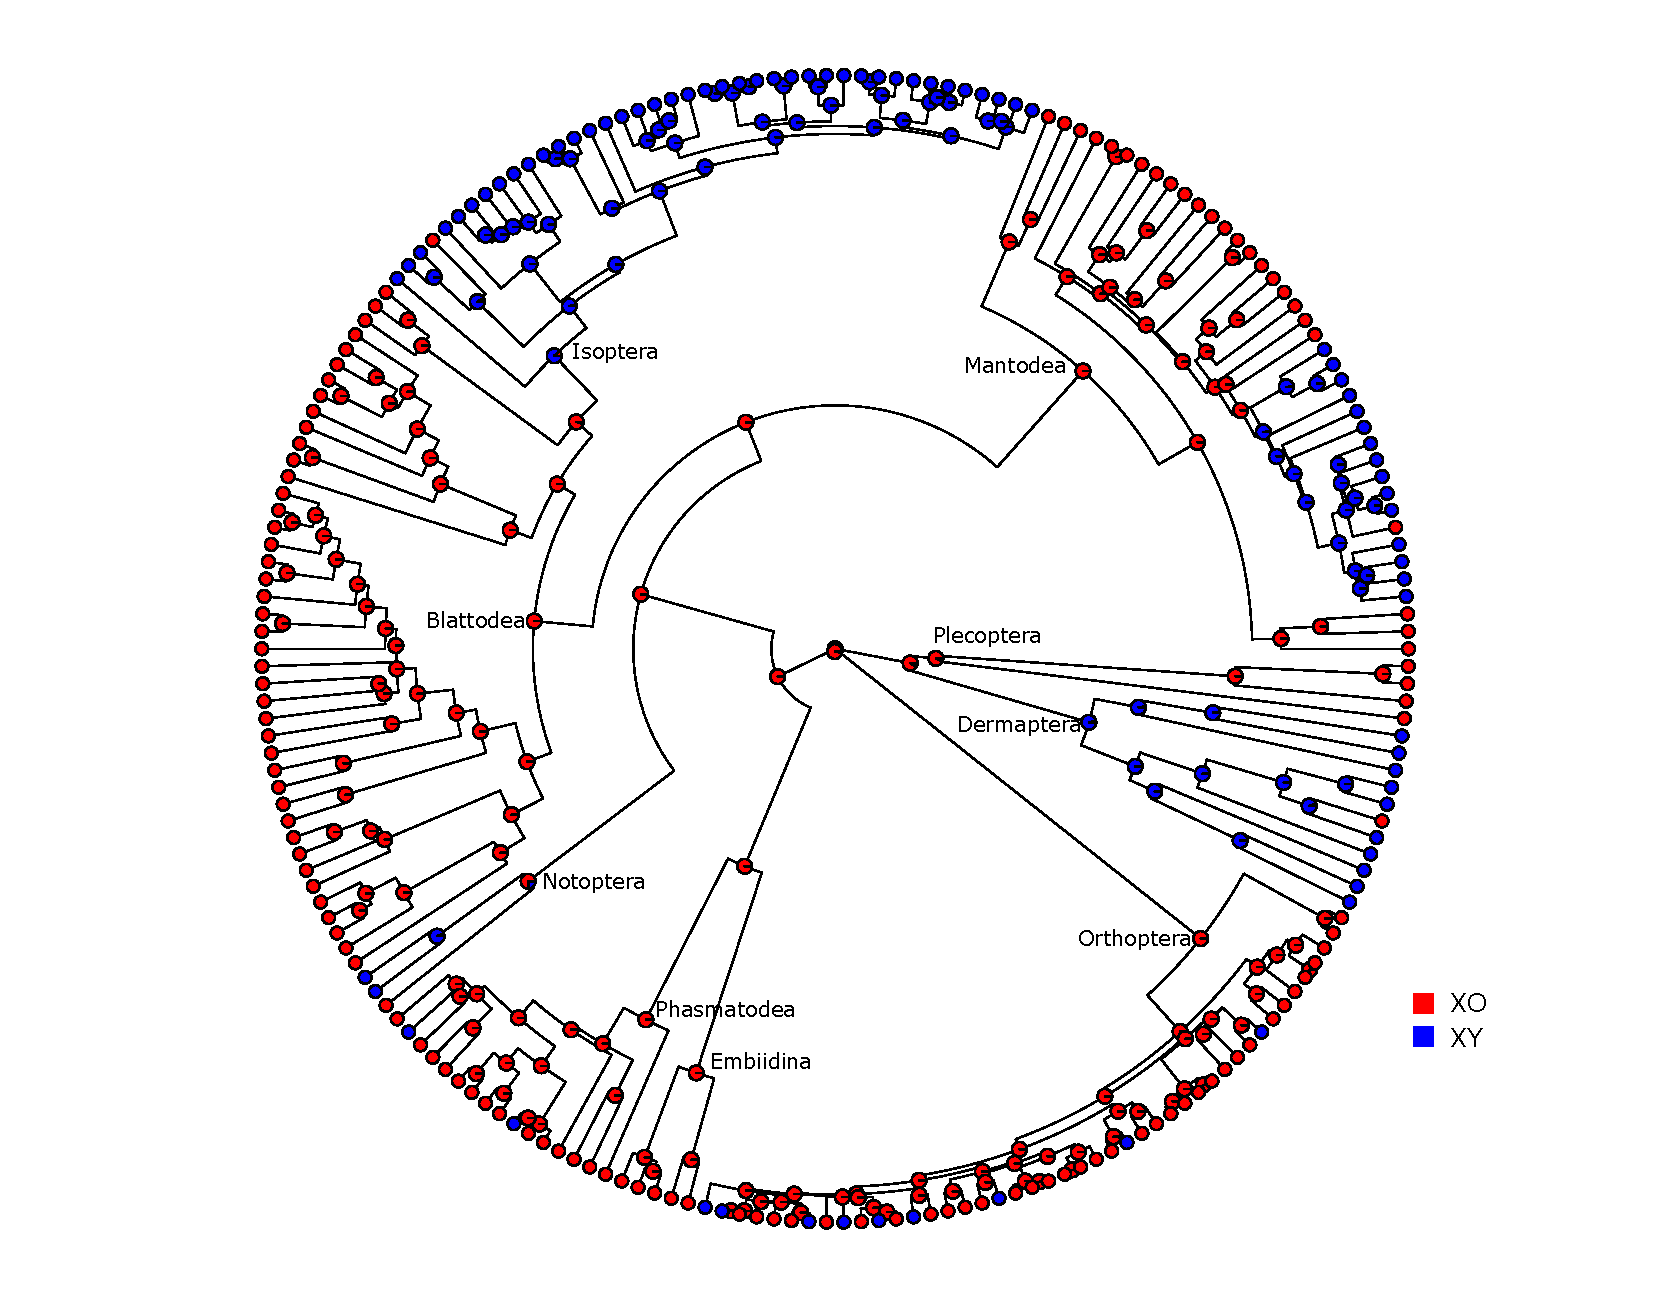
\includegraphics[width=1\textwidth]{sex_asr_plot.pdf}
\caption{Ancestral states reconstruction of the sex chromosome systems. 
This is a single tree of the posterior distribution. 
Red colour represents the XO sex chromosome system and blue colour represents the XY sex chromosome system. Order names are marked at the origin of each order. 
The probabilities of each sex chromosome system as being the ancestral state is given by the respective coloured portion of the pie charts at each node. 
Tip colours represent the current state of the sex chromosome system.}
\label{fig:sex.asr.plot}
\end{figure}

\newpage
\begin{figure}[h!]
\centering 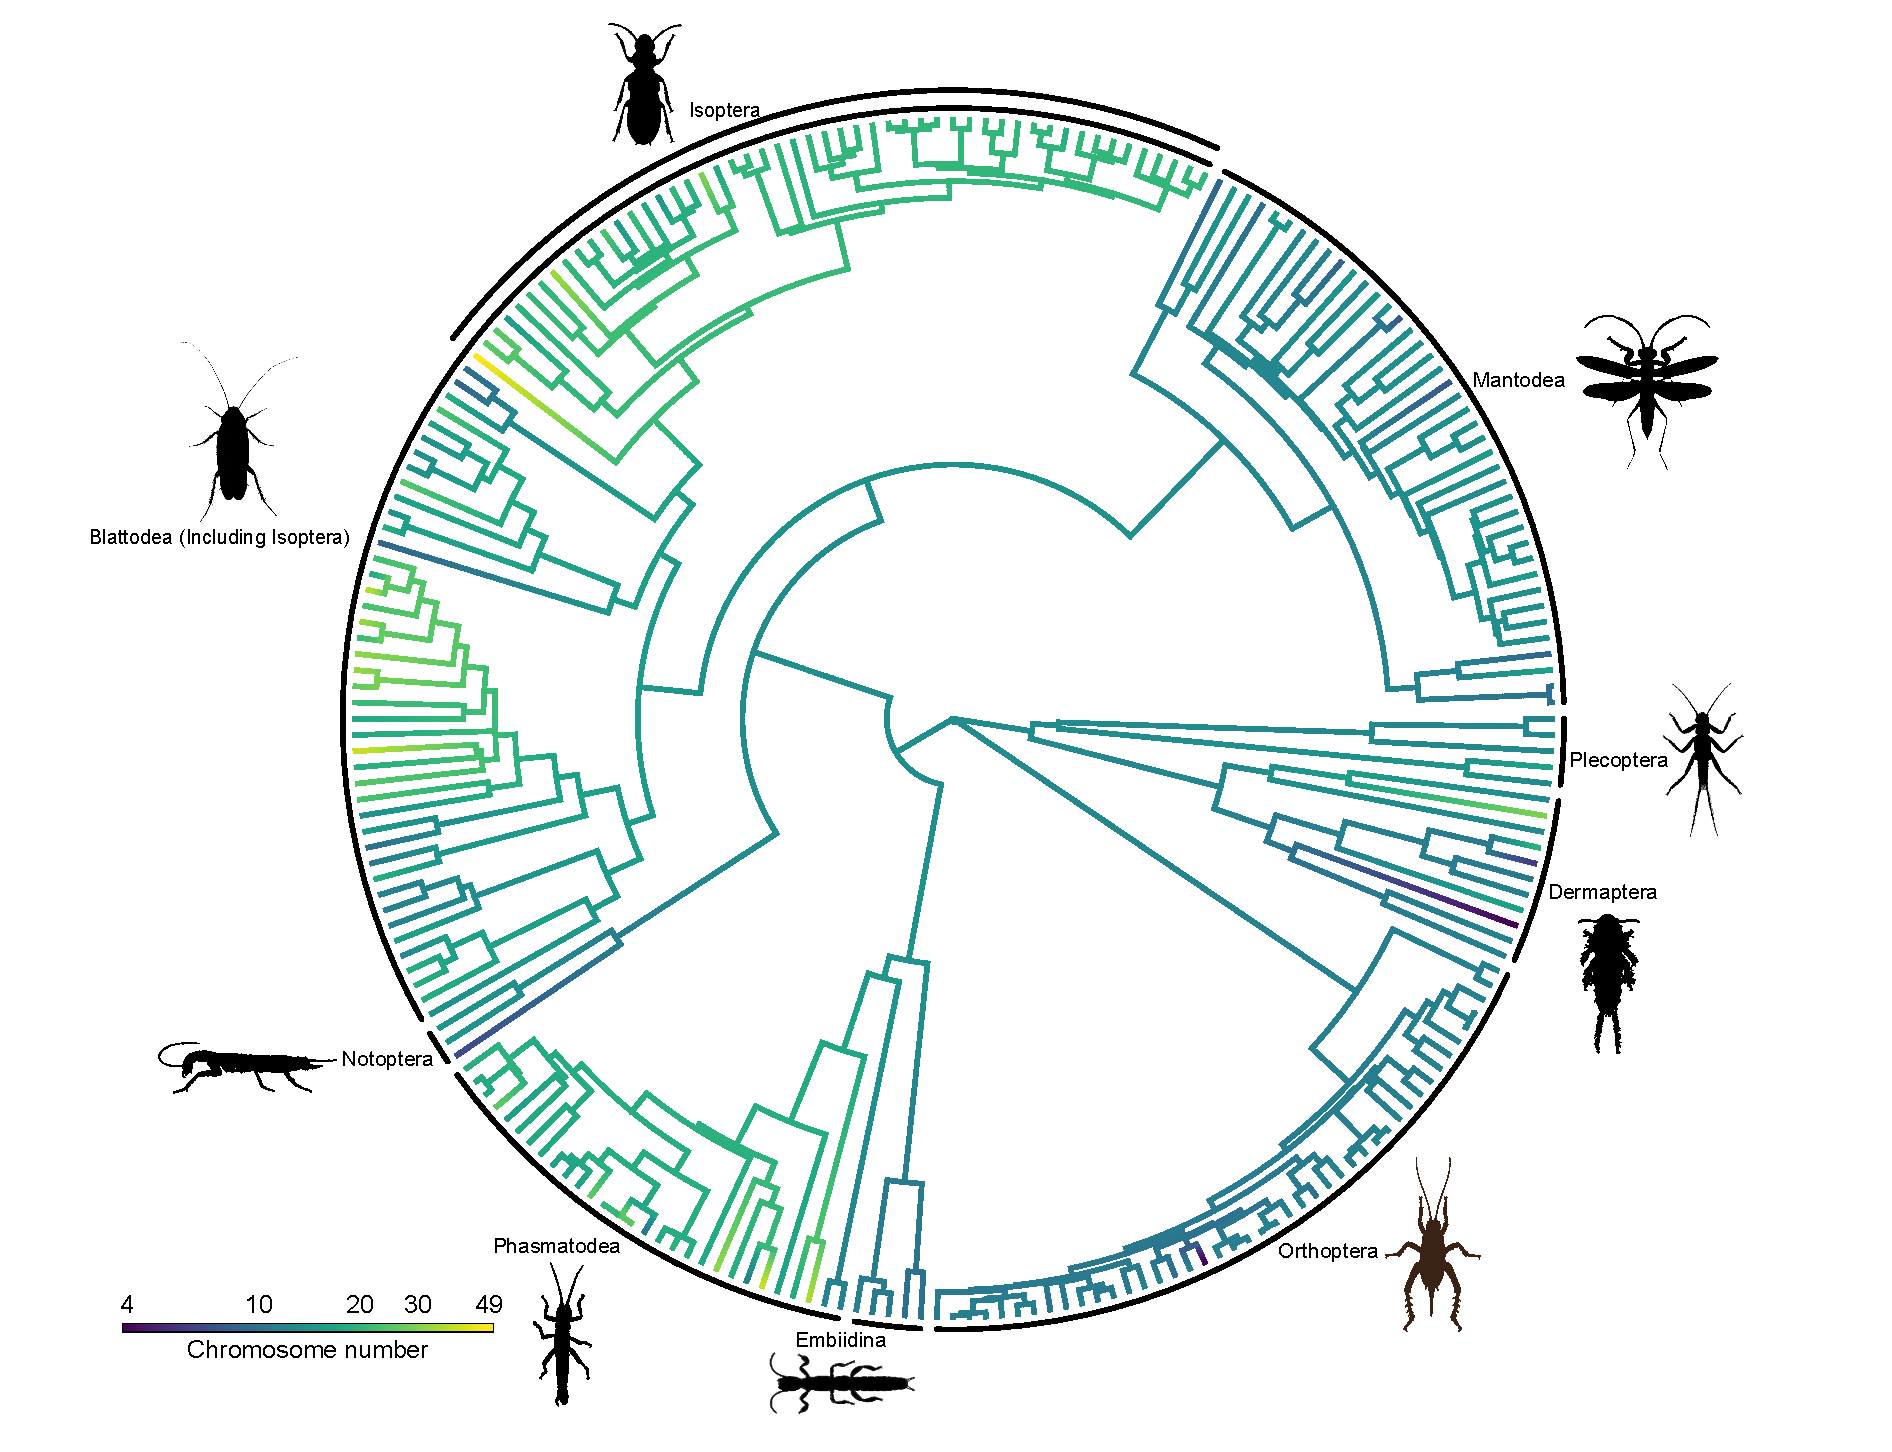
\includegraphics[width=1\textwidth]{phyloplot.pdf}
\caption{One of the 100 trees from the posterior distribution with taxonomy and chromosome number displayed. 
The solid black line indicates the tips included in each order. 
Branches are coloured according to ancestral state estimates under a Brownian motion model. }
\label{fig:phyloplot}
\end{figure}


\begin{figure}[h!]
\centering 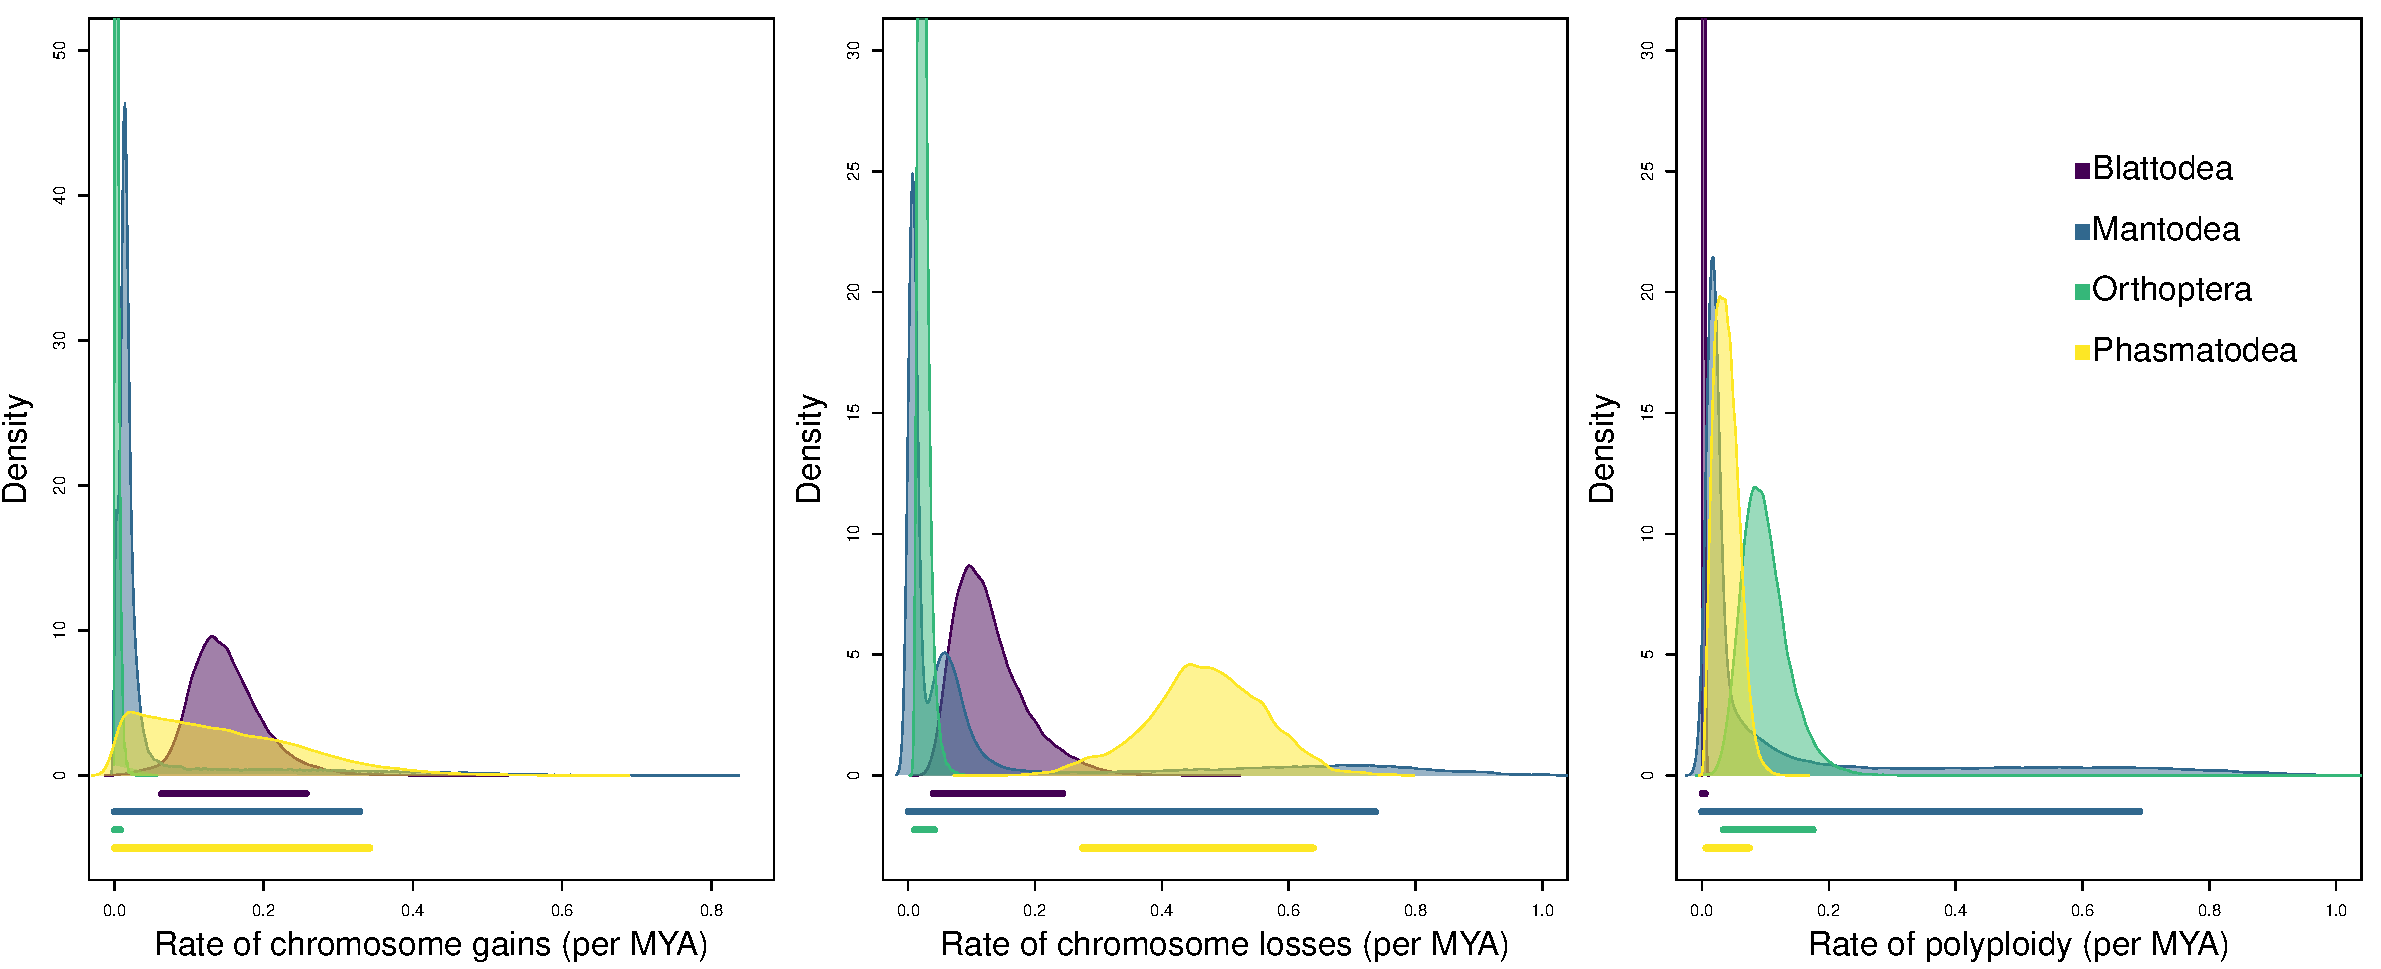
\includegraphics[width=1\textwidth]{order_rates_95HPD.pdf}
\caption{Rates of chromosome fusion, fission, and polyploidy of four orders in the insect clade Polyneoptera. 
The y-axis is shortened to show the spread of these rates. 
The bars below each distribution indicates the 95\% HPD interval.}
\label{fig:order.rates.95HPD}
\end{figure}


\begin{figure}[h!]
\centering 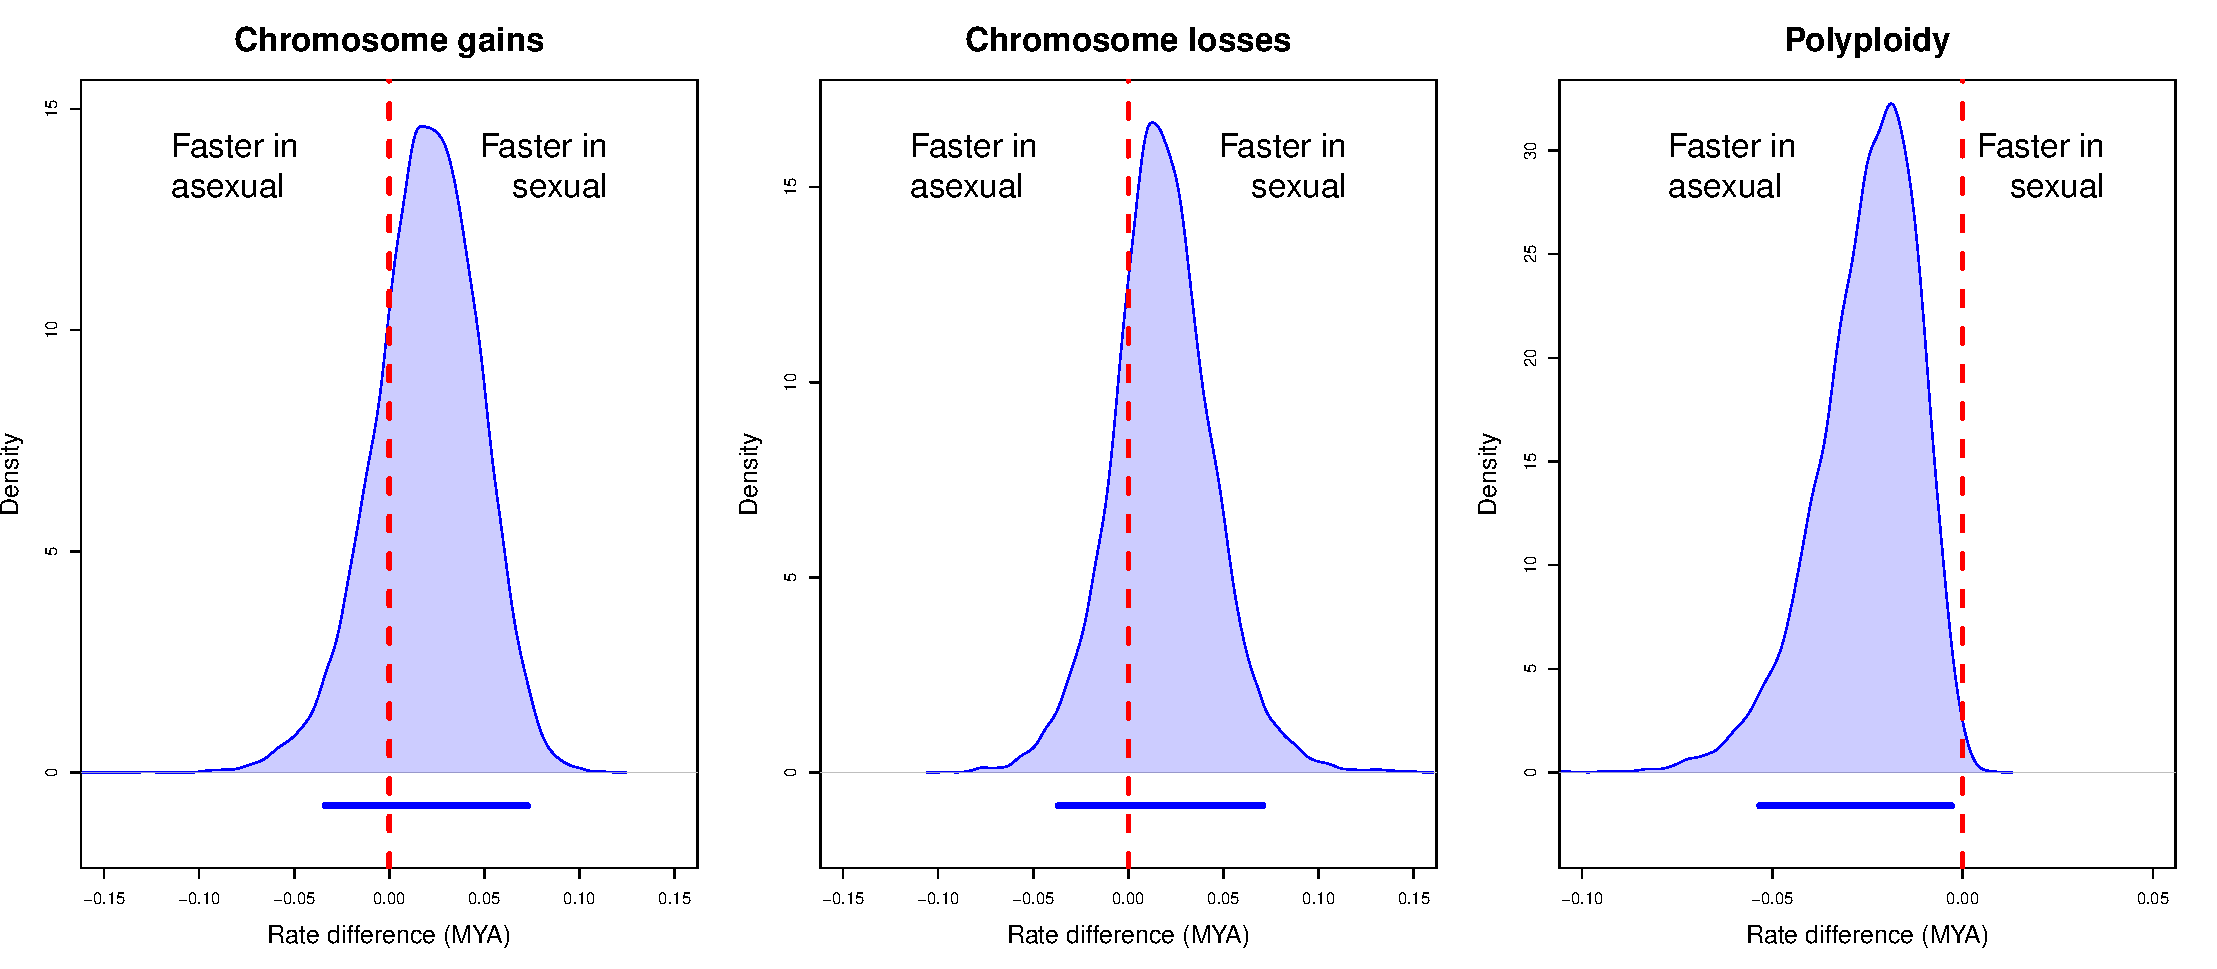
\includegraphics[width=1\textwidth]{phas_plot.pdf}
\caption{Rates of chromosome evolution in sexual and asexual lineages in Phasmatodea. 
Bars below the plot indicates the 95\% HPD interval}
\label{fig:phas.plot}
\end{figure}

%%%%%%%%%%%%
%% Tables %%
%%%%%%%%%%%%
\newpage
\begin{table}[!ht]
\small
\centering
\begin{tabular}{llcccccc}
\hline
\multirow{2}{*}{Order} &
  \multirow{2}{*}{Genera} &
  \multicolumn{2}{c}{\begin{tabular}[c]{@{}c@{}}Mean number of \\ autosomes\end{tabular}} &
  \multirow{2}{*}{\begin{tabular}[c]{@{}c@{}}Evidence \\ supports\end{tabular}} &
  \multicolumn{2}{c}{\begin{tabular}[c]{@{}c@{}}Mean number of \\ chromosomes\end{tabular}} &
  \multirow{2}{*}{\begin{tabular}[c]{@{}c@{}}Evidence\\  supports\end{tabular}} \\ \cline{3-4} \cline{6-7}
            &                              & XO   & XY   &        & XY   & multi &         \\ \hline
Dermaptera  & \textit{Forficula (14)}      & -    & 11   & -      & 12   & 12.8  & fission \\
Dermaptera  & \textit{Nala (3)}            & -    & 17.5 & -      & 18.5 & 19    & fission \\
Dermaptera  & \textit{Nesogaster (2)}      & 10   & -    & -      & -    & 11    & -       \\
Mantodea    & \textit{Deiphobe (2)}        & 9    & -    & -      & -    & 14    & -       \\
Orthoptera  & \textit{Aleuas (6)}          & 9    & 9.2  & -      & 10.2 & -     & -       \\
Orthoptera  & \textit{Dichroplus (35)}     & 10.7 & 8.7  & fusion & 9.7  & 11    & fission \\
Orthoptera  & \textit{Diponthus (7)}       & 10.5 & 10   & -      & 11   & -     & -       \\
Orthoptera  & \textit{Eurotettix (5)}      & -    & 10   & -      & 11   & 11    & -       \\
Orthoptera  & \textit{Gryllotalpa (5)}     & 9.7  & 5    & fusion & 6    & -     & -       \\
Orthoptera  & \textit{Isophya (25)}        & 15   & 14   & fusion & 15   & -     & -       \\
Orthoptera  & \textit{Leiotettix (10)}     & 11   & 8    & fusion & 9    & 7.5   & fusion  \\
Orthoptera  & \textit{Scotussa (8)}        & 10.6 & 8.5  & fusion & 9.5  & 11    & fission \\
Orthoptera  & \textit{Scyllina (3)}        & 11   & 10   & fusion & 11   & -     & -       \\
Orthoptera  & \textit{Tetrixocephalus (5)} & 11   & 10   & fusion & 11   & -     & -       \\
Orthoptera  & \textit{Xyleus (9)}          & 11   & 10   & fusion & 11   & -     & -       \\
Orthoptera  & \textit{Zoniopoda (6)}       & 11   & 10   & fusion & 11   & -     & -       \\
Phasmatodea & \textit{Didymuria (10)}      & 17.6 & 14.4 & fusion & 15.4 & -     & -       \\
Phasmatodea & \textit{Isagoras (3)}        & 18   & 16   & fusion & 17   & -     & -       \\
Phasmatodea & \textit{Leptynia (5)}        & 18.2 & 17   & fusion & 18   & -     & -       \\
Phasmatodea & \textit{Podacanthus (3)}     & 17   & 13   & fusion & 14   & -     & -       \\
Phasmatodea & \textit{Prisopus (2)}        & 24   & 13   & fusion & 14   & -     & -       \\
Plecoptera  & \textit{Perla (7)}           & 9.5  & 4    & fusion & 5    & 12.8  & fission \\ \hline
\end{tabular}
\caption{Chromosome number and sex chromosome systems. In each genus, we report the mean number of autosomes for all species having XO and XY sex chromosome systems and the mean number of chromosomes for all species having XY and complex sex chromosome systems. Evidence supports column states whether the given chromosome numbers supports fusion or fission as an important process in transition between these sex chromosome systems. Negative (-) symbol indicates a distribution of chromosome number that is uninformative or does not support a given mechanism.}
\label{tab:fusions}
\end{table}

\vspace*{-10pt}

\noindent 

%%%%%%%%%% Insert bibliography here %%%%%%%%%%%%%%
\newpage
\begin{thebibliography}{99}

\bibitem{flemming1882}
Flemming W. 
 Zellsubstanz, kern und zelltheilung. Leipzig, Germany: Vogel; 1882.

\bibitem{garagna1995}
Garagna S, Broccoli D, Redi CA, Searle JB, Cooke HJ, Capanna E.
 Robertsonian metacentrics of the house mouse lose telomeric sequences
  but retain some minor satellite DNA in the pericentromeric area.
 Chromosoma. 1995;103(10):685--692.

\bibitem{gordon2011mechanisms}
Gordon JL, Byrne KP, Wolfe KH.
 Mechanisms of chromosome number evolution in yeast.
 PLoS genetics. 2011;7(7):e1002190.

\bibitem{miga2016}
Miga KH.
 Chromosome-specific centromere sequences provide an estimate of the
  ancestral chromosome 2 fusion event in hominin genomes.
 Journal of Heredity. 2016;108(1):45--52.

\bibitem{moretti1984}
Moretti A, Sabato S.
 Karyotype evolution by centromeric fission in Zamia (Cycadales).
 Plant Systematics and Evolution. 1984;146(3-4):215--223.

\bibitem{hornsey1973}
Hornsey K.
 The occurrence of hexaploid plants among autotetraploid populations
  of sugar beet,(Beta Vulgaris L.) and the production of tetraploid progeny
  using a diploid pollinator.
 Caryologia. 1973;26(2):225--228.

\bibitem{beccak1970}
Be{\c{c}}ak ML, Denaro L, Be{\c{c}}ak W.
 Polyploidy and mechanisms of karyotypic diversification in Amphibia.
 Cytogenetic and Genome Research. 1970;9(4):225--238.

\bibitem{lockstone2007}
Lockstone H, Harris L, Swatton J, Wayland M, Holland A, Bahn S.
 Gene expression profiling in the adult Down syndrome brain.
 Genomics. 2007;90(6):647--660.

\bibitem{williams2008aneuploidy}
Williams BR, Prabhu VR, Hunter KE, Glazier CM, Whittaker CA, Housman DE, et~al.
 Aneuploidy affects proliferation and spontaneous immortalization in
  mammalian cells.
 Science. 2008;322(5902):703--709.

\bibitem{sun2013dosage}
Sun L, Johnson AF, Donohue RC, Li J, Cheng J, Birchler JA.
 Dosage compensation and inverse effects in triple X metafemales of
  Drosophila.
 Proceedings of the National Academy of Sciences.
  2013;110(18):7383--7388.

\bibitem{stebbins1958}
Stebbins GL.
 Longevity, habitat, and release of genetic variability in the higher
  plants.
 In: Cold Spring Harbor Symposia on Quantitative Biology. vol.~23.
  Cold Spring Harbor Laboratory Press; 1958. p. 365--378.

\bibitem{dumont2017req}
Dumont BL.
 Variation and Evolution of the Meiotic Requirement for Crossing Over
  in Mammals.
 Genetics. 2017;205(1):155--168.

\bibitem{ross2015}
Ross L, Blackmon H, Lorite P, Gokhman VE, Hardy NB.
 Recombination, chromosome number and eusociality in the
  {H}ymenoptera.
 Journal of Evolutionary Biology. 2015;28(1):105--116.

\bibitem{sherman1979}
Sherman PW.
 Insect chromosome numbers and eusociality.
 American Naturalist. 1979;113:925--935.

\bibitem{kitano2012}
Kitano J, Peichel CL.
 Turnover of sex chromosomes and speciation in fishes.
 Environmental biology of fishes. 2012;94(3):549--558.

\bibitem{blackmon2015bioessay}
Blackmon H, Demuth JP.
 The fragile Y hypothesis: Y chromosome aneuploidy as a selective
  pressure in sex chromosome and meiotic mechanism evolution.
 BioEssays. 2015;37(9):942--950.

\bibitem{blackmon2014}
Blackmon H, Demuth JP.
 Estimating tempo and mode of Y chromosome turnover: explaining Y
  chromosome loss with the fragile Y hypothesis.
 Genetics. 2014;197(2):561--572.

\bibitem{dumont2017par}
Dumont BL.
 Meiotic consequences of genetic divergence across the murine
  pseudoautosomal region.
 Genetics. 2017;205(3):1089--1100.

\bibitem{white1973}
White MJD.
 Animal Cytology and Evolution.
 London, UK: Cambridge University Press; 1973.

\bibitem{wodsedalek1916}
Wodsedalek J.
 Causes of sterility in the mule.
 The Biological Bulletin. 1916;30(1):1--56.

\bibitem{britton1990robertsonian}
Britton-Davidian J, Sonjaya H, Catalan J, Cattaneo-Berrebi G.
 Robertsonian heterozygosity in wild mice: fertility and transmission
  rates in Rb (16.17) translocation heterozygotes.
 Genetica. 1990;80(3):171--174.

\bibitem{ratomponirina1988}
Ratomponirina C.
 Synaptonemal complexes in Robertsonian translocation heterozygous in
  lemurs.
 Kew Chromosomes. 1988.

\bibitem{lachowska1998}
Lachowska D, Holecova M, Rozek M.
 Karyotypic data on weevils (Coleoptera, Curculionidae).
 FOLIA BIOLOGICA-KRAKOW-. 1998;46:129--136.

\bibitem{blackmon2016}
Blackmon H, Ross L, Bachtrog D.
 Sex determination, sex chromosomes, and karyotype evolution in
  insects.
 Journal of Heredity. 2016;108(1):78--93.

\bibitem{TOS2014}
{Tree of Sex Consortium}.
 Tree of Sex: a database of sexual systems.
 Scientific Data. 2014;1.

\bibitem{smith2018phyphlawd}
Smith SA, Brown JW.
 Constructing a broadly inclusive seed plant phylogeny.
 American journal of botany. 2018;105(3):302--314.

\bibitem{blackmon2015evobir}
Blackmon H, Adams R. EvobiR: tools for comparative analyses and teaching
  evolutionary biology. 2015.

\bibitem{katoh2013mafft}
Katoh K, Standley DM.
 MAFFT multiple sequence alignment software version 7: improvements in
  performance and usability.
 Molecular biology and evolution. 2013;30(4):772--780.

\bibitem{castresana2000gblocks}
Castresana J.
 Selection of conserved blocks from multiple alignments for their use
  in phylogenetic analysis.
 Molecular biology and evolution. 2000;17(4):540--552.

\bibitem{aberer2012roguetaxa}
Aberer AJ, Krompass D, Stamatakis A.
 Pruning rogue taxa improves phylogenetic accuracy: an efficient
  algorithm and webservice.
 Systematic biology. 2012;62(1):162--166.

\bibitem{rabosky2015b}
Rabosky DL.
 No Substitute for Real Data: a Cautionary Note on the Use of
  Phylogenies from Birth--Death Polytomy Resolvers for Downstream Comparative
  Analyses.
 Evolution. 2015;69(12):3207--3216.

\bibitem{stamatakis2014raxml}
Stamatakis A.
 RAxML version 8: a tool for phylogenetic analysis and post-analysis
  of large phylogenies.
 Bioinformatics. 2014;30(9):1312--1313.

\bibitem{miller2010cipres}
Miller MA, Pfeiffer W, Schwartz T.
 Creating the CIPRES Science Gateway for inference of large
  phylogenetic trees.
 In: Gateway Computing Environments Workshop (GCE), 2010. Ieee; 2010.
  p. 1--8.

\bibitem{maddison2018mesquite}
Maddison WP, Maddison DR.
 Mesquite: a modular system for evolutionary analysis. Version 3.51.
 http://mesquiteproject.org. 2018.

\bibitem{bouckaert2014beast}
Bouckaert R, Heled J, K{\"u}hnert D, Vaughan T, Wu CH, Xie D, et~al.
 BEAST 2: a software platform for Bayesian evolutionary analysis.
 PLoS computational biology. 2014;10(4):e1003537.

\bibitem{misof2014phylogenomics}
Misof B, Liu S, Meusemann K, Peters RS, Donath A, Mayer C, et~al.
 Phylogenomics resolves the timing and pattern of insect evolution.
 Science. 2014;346(6210):763--767.

\bibitem{rambaut2018tracer}
Rambaut A, Drummond AJ, Xie D, Baele G, Suchard MA.
 Posterior summarisation in Bayesian phylogenetics using Tracer 1.7.
 Syst Biol. 2018;10.

\bibitem{sanderson2008}
Sanderson MJ, Boss D, Chen D, Cranston KA, Wehe A.
 The PhyLoTA Browser: processing GenBank for molecular phylogenetics
  research.
 Systematic Biology. 2008;57(3):335--346.

%\bibitem{fitzjohn2012}
%FitzJohn RG.
% Diversitree: comparative phylogenetic analyses of diversification in
%  {R}.
% Methods in Ecology and Evolution. 2012;3(6):1084--1092.

\bibitem{glick2014chromevol}
Glick L, Mayrose I.
 ChromEvol: assessing the pattern of chromosome number evolution and
  the inference of polyploidy along a phylogeny.
 Molecular Biology and Evolution. 2014;31(7):1914--1922.

\bibitem{mayrose2009chromevol}
Mayrose I, Barker MS, Otto SP.
 Probabilistic models of chromosome number evolution and the inference
  of polyploidy.
 Systematic Biology. 2009;59(2):132--144.

\bibitem{zenil2018chromploid}
Zenil-Ferguson R, Burleigh JG, Ponciano JM.
 chromploid: An R package for chromosome number evolution across the
  plant tree of life.
 Applications in plant sciences. 2018;6(3).
 
 \bibitem{freyman2018}
Freyman WA, H{\"o}hna S.
 Cladogenetic and Anagenetic Models of Chromosome Number Evolution: a
  {B}ayesian Model Averaging Approach.
 Systematic Biology. 2018;67:195--215.

\bibitem{blackmon2019meiotic}
Blackmon H, Justison J, Mayrose I, Goldberg EE.
 Meiotic drive shapes rates of karyotype evolution in mammals.
 Evolution. 2019;.

\bibitem{kidwell2002transposable}
Kidwell MG.
 Transposable elements and the evolution of genome size in eukaryotes.
 Genetica. 2002;115(1):49--63.

\bibitem{bennetzen2005mechanisms}
Bennetzen JL, Ma J, Devos KM.
 Mechanisms of recent genome size variation in flowering plants.
 Annals of botany. 2005;95(1):127--132.

\bibitem{gregory2019}
Gregory TR. Animal Genome Size Database; 2019.
 Accessed: 2019-07-08.
 \url{http://www.genomesize.com}.
 
\bibitem{johnston2019}
Johnston JS, Bernardini A, Hjelmen CE. 2019. 
Genome Size Estimation and Quantitative Cytogenetics in Insects. In Insect Genomics, pp. 15-26. Springer.

\bibitem{hanrahan2011}
Hanrahan SJ, Johnston JS. 2011. 
New genome size estimates of 134 species of arthropods. Chromosome Research 19: 809-823.

\bibitem{R-citation}
{R Core Team}. R: A Language and Environment for Statistical Computing.
 Vienna, Austria; 2019.
 Available from: \url{https://www.R-project.org/}.
 
 \bibitem{phylolm}
Ho LST, Ane C.
 A linear-time algorithm for Gaussian and non-Gaussian trait evolution
  models.
 Systematic Biology. 2014;63:397--408.

\bibitem{Paradis2018}
Paradis E, Schliep K.
 ape 5.0: an environment for modern phylogenetics and evolutionary
  analyses in {R}.
 Bioinformatics. 2018;35:526--528.

\bibitem{revell2012phytools}
Revell LJ.
 phytools: an R package for phylogenetic comparative biology (and
  other things).
 Methods in Ecology and Evolution. 2012;3(2):217--223.

\bibitem{charlesworth1980}
Charlesworth D, Charlesworth B.
 Sex differences in fitness and selection for centric fusions between
  sex-chromosomes and autosomes.
 Genetics Research. 1980;35(2):205--214.

\bibitem{steinemann2005}
Steinemann S, Steinemann M.
 Y chromosomes: born to be destroyed.
 Bioessays. 2005;27(10):1076--1083.

\bibitem{meisel2019x}
Meisel RP, Delclos PJ, Wexler JR.
 The X chromosome of the German cockroach, Blattella germanica, is
  homologous to a fly X chromosome despite 400 million years divergence.
 BMC biology. 2019;17(1):1--14.

\bibitem{bush1977rapid}
Bush GL, Case S, Wilson A, Patton J.
 Rapid speciation and chromosomal evolution in mammals.
 Proceedings of the National Academy of Sciences.
  1977;74(9):3942--3946.

\bibitem{sved2016}
Sved JA, Chen Y, Shearman D, Frommer M, Gilchrist AS, Sherwin WB.
 Extraordinary conservation of entire chromosomes in insects over long
  evolutionary periods.
 Evolution. 2016;70(1):229--234.
 
 \bibitem{li2018multiple}
Li Z, Tiley GP, Galuska SR, Reardon CR, Kidder TI, Rundell RJ, et~al.
Multiple large-scale gene and genome duplications during the evolution of hexapods.
Proceedings of the National Academy of Sciences.
2018;115(18):4713--4718.

%\bibitem{ohno}
%Ohno S.
% Evolution by gene duplication.
% New York, USA: Springer Science; 1970.

\bibitem{white1978}
White MJD.
 Chain processes in chromosomal speciation.
 Systematic Biology. 1978;27(3):285--298.
 
 \bibitem{liehr2017new}
Liehr T, Buleu O, Karamysheva T, Bugrov A, Rubtsov N.
 New insights into phasmatodea chromosomes.
Genes. 2017;8(11):327.

\bibitem{rockman2002}
Rockman MV, Rowell DM.
 Episodic chromosomal evolution in \emph{{P}lanipapillus}
  ({O}nychophora: {P}eripatopsidae): a phylogenetic approach to evolutionary
  dynamics and speciation.
 Evolution. 2002;56(1):58--69.

\bibitem{mccann2016}
McCann J, Schneeweiss GM, Stuessy TF, Villasenor JL, Weiss-Schneeweiss H.
 The impact of reconstruction methods, phylogenetic uncertainty and
  branch lengths on inference of chromosome number evolution in American
  daisies (Melampodium, Asteraceae).
 PloS one. 2016;11(9):e0162299.

\bibitem{deoliveira}
De~Oliveira IG, Moraes AP, De~Almeida EM, de~Assis FNM, Cabral JS, De~Barros F,
  et~al.
 Chromosomal evolution in Pleurothallidinae (Orchidaceae:
  Epidendroideae) with an emphasis on the genus Acianthera: chromosome numbers
  and heterochromatin.
 Botanical journal of the Linnean Society. 2015;178(1):102--120.

\bibitem{zenil2017}
Zenil-Ferguson R, Ponciano JM, Burleigh JG.
 Testing the Association of Phenotypes with Polyploidy: An Example
  Using Herbaceous and Woody Eudicots.
 Evolution. 2017;71:1138--1148.

\bibitem{lokki1980polyploidy}
Lokki J, Saura A.
 Polyploidy in insect evolution.
 In: Polyploidy. New York, USA: Springer; 1980. p. 277--312.

\bibitem{carbone2014gibbon}
Carbone L, Harris RA, Gnerre S, Veeramah KR, Lorente-Galdos B, Huddleston J,
  et~al.
 Gibbon genome and the fast karyotype evolution of small apes.
 Nature. 2014;513(7517):195.

 \bibitem{hughes1950chromosomes}
Hughes-Schrader S.
 The chromosomes of mantids (Orthoptera: Manteidae) in relation to
  taxonomy.
 Chromosoma. 1950;4(1):1--55.

\bibitem{blackman1995sex}
Blackman RL, Leather S, Hardie J.
 Sex determination in insects.
 Insect Reproduction. 1995;p. 57--94.

\bibitem{luykx1990cytogenetic}
Luykx P.
 A cytogenetic survey of 25 species of lower termites from Australia.
Genome. 1990;33(1):80--88.

\bibitem{bergamaschi2007karyology}
Bergamaschi S, Dawes-Gromadzki TZ, Scali V, Marini M, Mantovani B.
 Karyology, mitochondrial DNA and the phylogeny of Australian
  termites.
Chromosome Research. 2007;15(6):735.

\bibitem{white1976}
White M.
\newblock Insecta 2. Blattodea, Mantodea, Isoptera, Grylloblattodea,
  Phasmatodea, Dermaptera and Embioptera.
\newblock Schweizerbart'sche Verlagsbuchhandlung; 1976.

\bibitem{hughes1959}
Hughes-Schrader S.
 On the cytotaxonomy of phasmids (Phasmatodea).
 Chromosoma. 1959;10(1-6):268--277.

\bibitem{baker1986}
Baker RJ, Bickham JW.
 Speciation by monobrachial centric fusions.
 Proceedings of the National Academy of Sciences.
  1986;83(21):8245--8248.

\bibitem{white}
White MJD.
 Modes of speciation.
 San Francisco, USA: WH Freeman; 1978.
 
\bibitem{rieseberg2001}
Rieseberg LH.
Chromosomal rearrangements and speciation.
Trends in ecology \& evolution. 2001;16(7):351--358

\bibitem{stebbins1971}
Stebbins GL, et~al.
 Chromosomal evolution in higher plants.
 Chromosomal evolution in higher plants. 1971;

\end{thebibliography}


\end{document}

